% BLM308 Veri Madenciliği - Beamer Sunumu
\documentclass[aspectratio=169,12pt]{beamer}

\usetheme{Madrid}
\usecolortheme{default}
\usepackage[utf8]{inputenc}
\usepackage[T1]{fontenc}
\usepackage[turkish]{babel}
\usepackage{graphicx}
\usepackage{booktabs}
\usepackage{hyperref}

\graphicspath{{../reports/figures/}}

\title[Ürün İade Tahmini]{Çevrimiçi Alışveriş Ürün İade Tahmini}
\subtitle{BLM308 Veri Madenciliği Final Projesi}
\author{Emre Kaya}
\institute{Öğrenci No: 231041045 \quad Mayıs 2026\\ \url{https://github.com/emrekayy/blm308-urun-iade-tahmini}}
\date{}

\begin{document}

% 1. Title
\begin{frame}
    \titlepage
\end{frame}

% 2. Problem
\begin{frame}{Problem Tanımı}
    \begin{itemize}
        \item Bir e-ticaret siparişinin/ürünün iade edilip edilmeyeceğini tahmin etmek
        \item İkili hedef: \texttt{return\_status} (0 = iade yok, 1 = iade var)
        \item Amaç: iade kaynaklı operasyonel maliyeti azaltmak ve müşteri deneyimini iyileştirmek
    \end{itemize}
\end{frame}

% 3. Motivation
\begin{frame}{Motivasyon}
    \begin{itemize}
        \item İadeler lojistik ve yeniden stoklama maliyetlerini artırır
        \item Erken risk tespiti proaktif müşteri hizmetini destekler
        \item İçgörüler fiyatlandırma ve ürün kalitesi iyileştirmelerine rehberlik eder
    \end{itemize}
\end{frame}

% 4. Dataset
\begin{frame}{Veri Seti}
    \begin{itemize}
        \item Dosya: \texttt{product\_return\_prediction.csv}
        \item 1.500 kayıt; sütunlar: \texttt{order\_id}, \texttt{product\_id}, \texttt{price}, \texttt{rating}, \texttt{return\_status}
        \item Sınıf dağılımı: 0 = 1.094 (\%72,9), 1 = 406 (\%27,1)
        \item Eksik değer yok; kategori, indirim, teslimat sütunları yok
    \end{itemize}
\end{frame}

% 5. EDA
\begin{frame}{EDA Bulguları}
    \begin{columns}
        \column{0.55\textwidth}
        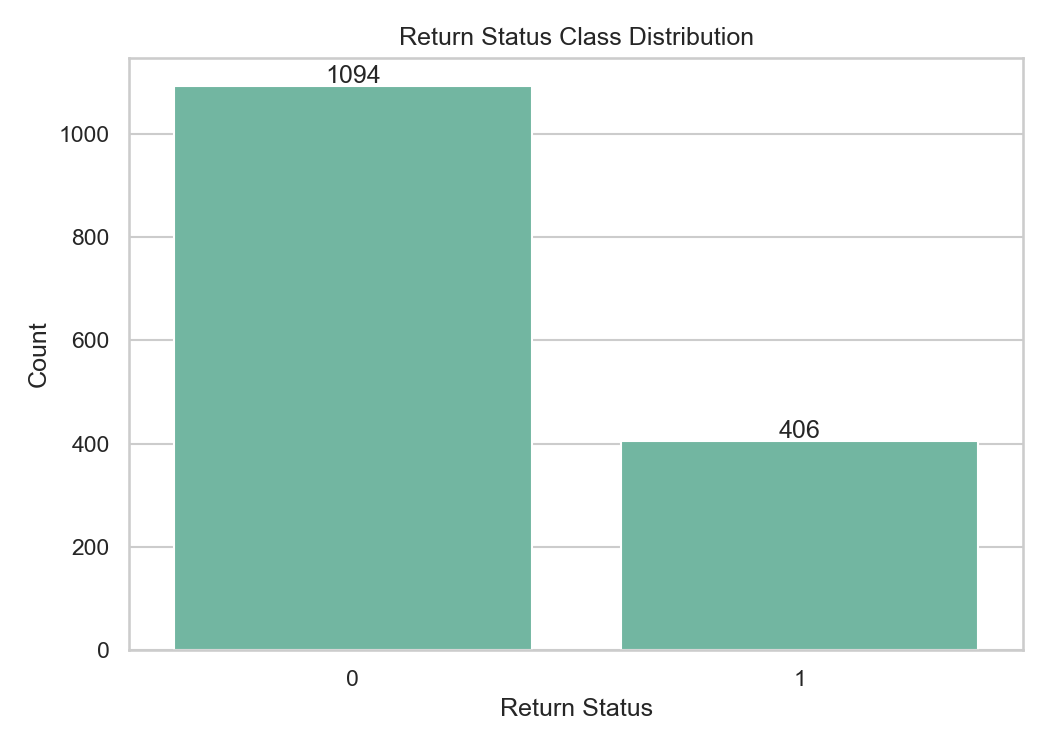
\includegraphics[width=\textwidth]{01_class_distribution.png}
        \column{0.45\textwidth}
        \small
        \begin{itemize}
            \item Dengesiz veri seti
            \item İade oranı $\approx$ \%27
            \item Azınlık sınıf: iade edilen siparişler
        \end{itemize}
    \end{columns}
\end{frame}

\begin{frame}{Fiyat ve Puan Kalıpları}
    \begin{columns}
        \column{0.5\textwidth}
        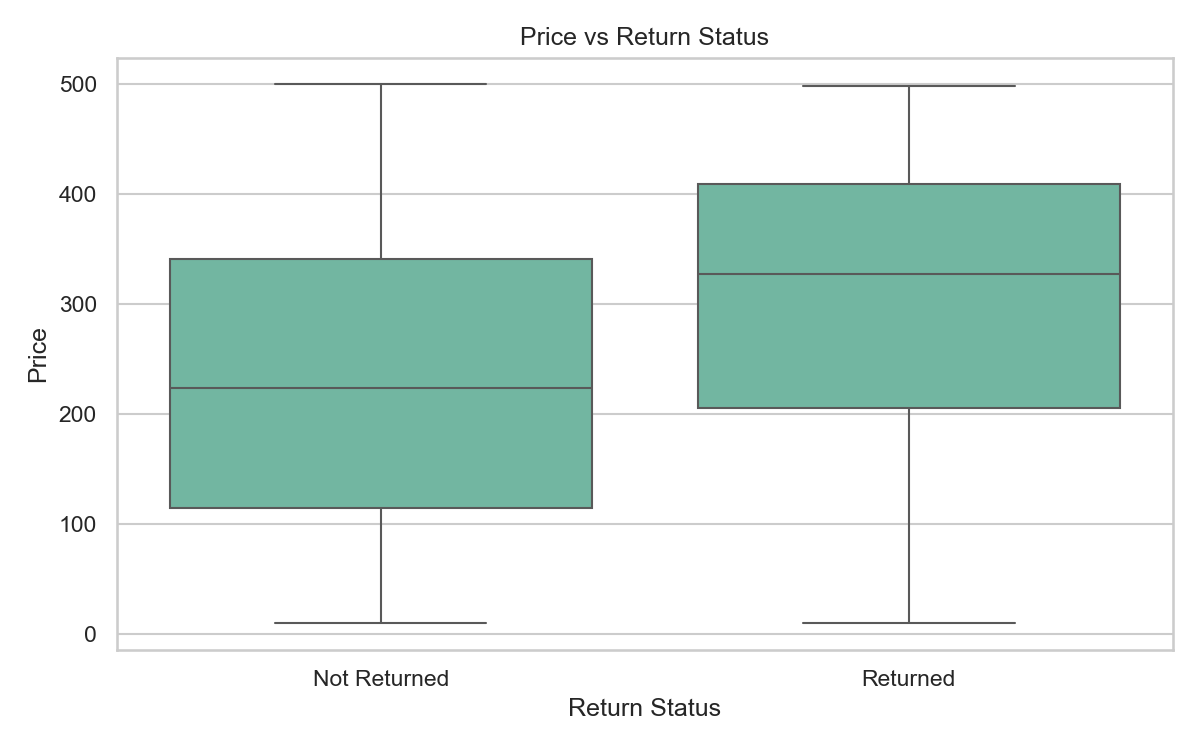
\includegraphics[width=\textwidth]{03_price_vs_return.png}
        \column{0.5\textwidth}
        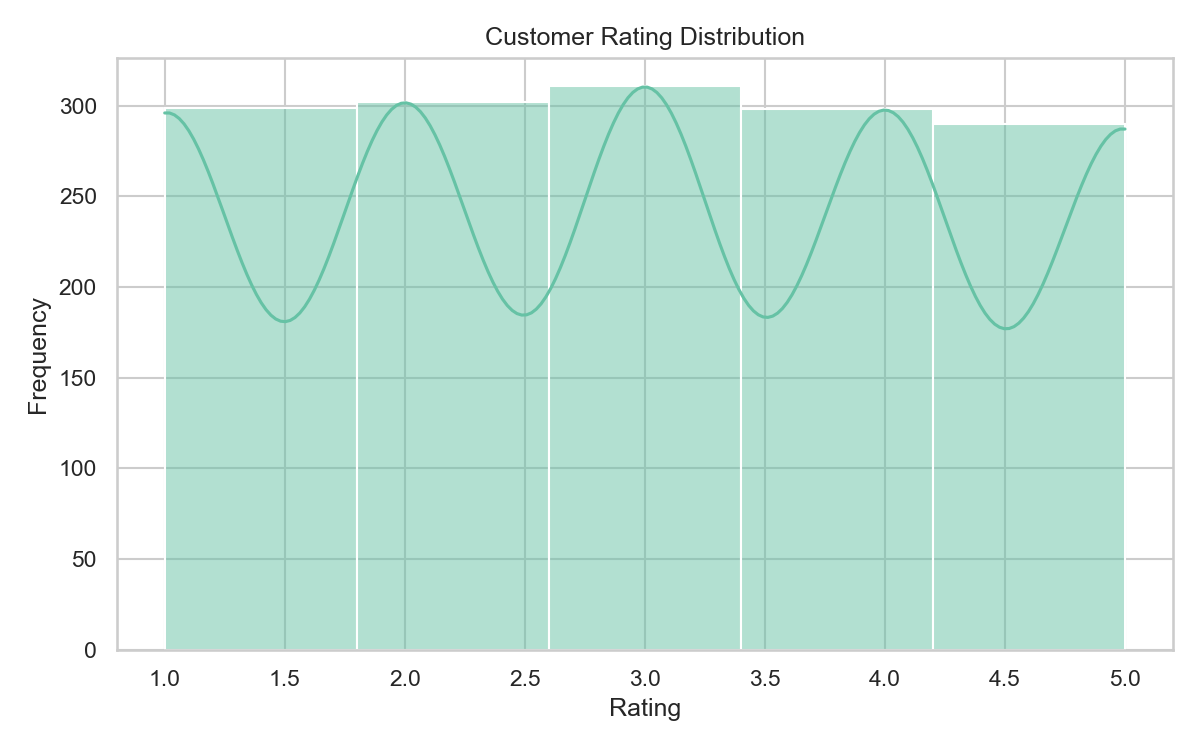
\includegraphics[width=\textwidth]{05_rating_distribution.png}
    \end{columns}
    \vspace{0.3cm}
    \small İade edilen siparişlerde ortalama fiyat daha yüksek; puanlar daha düşük.
\end{frame}

% 6. Preprocessing
\begin{frame}{Ön İşleme}
    \begin{itemize}
        \item \texttt{order\_id} çıkarıldı; \texttt{product\_id} ordinal kullanılmadı
        \item \texttt{product\_id\_frequency}: ürünün eğitim kümesindeki görülme sayısı
        \item \texttt{product\_return\_rate}: ürün iade oranı (yalnızca eğitim kümesi)
        \item Scaler yalnızca eğitimde fit; split encoding öncesinde (\%80/\%20)
        \item Özellikler: \texttt{price}, \texttt{rating}, frekans, iade oranı
    \end{itemize}
\end{frame}

% 7. Models
\begin{frame}{Seçilen Modeller}
    \begin{enumerate}
        \item Decision Tree (Karar Ağacı)
        \item Random Forest (Rastgele Orman)
        \item Logistic Regression (Lojistik Regresyon)
        \item Naive Bayes
        \item KNN
    \end{enumerate}
\end{frame}

% 8. Evaluation setup
\begin{frame}{Değerlendirme Kurulumu}
    \begin{itemize}
        \item 10 katmanlı Stratified CV --- \textbf{yalnızca eğitim kümesi} (1.200 kayıt)
        \item Ürün encoding her CV fold içinde yeniden hesaplandı
        \item Test kümesi (300 kayıt) yalnızca \textbf{bir kez} final değerlendirme
        \item Metrikler: Doğruluk, Kesinlik, Duyarlılık, F1, ROC-AUC
        \item Model seçimi: CV F1-skoru
    \end{itemize}
\end{frame}

% 9. Results
\begin{frame}{Sonuçlar (CV -- Eğitim Kümesi)}
    \footnotesize
    \begin{table}
        \centering
        \begin{tabular}{lcccc}
            \toprule
            Model & Doğruluk & F1 & ROC-AUC \\
            \midrule
            Random Forest & 0,672 & \textbf{0,307} & 0,533 \\
            Decision Tree & 0,628 & 0,282 & 0,517 \\
            Naive Bayes   & 0,663 & 0,279 & 0,577 \\
            KNN           & 0,669 & 0,266 & 0,520 \\
            Log. Reg.     & 0,668 & 0,265 & 0,571 \\
            \bottomrule
        \end{tabular}
    \end{table}
\end{frame}

% 10. Best model
\begin{frame}{En İyi Model: Random Forest}
    \textbf{Bağımsız test kümesi (300 kayıt):}
    \begin{itemize}
        \item Doğruluk: 0,6467 \quad Kesinlik: 0,2727
        \item Duyarlılık: 0,1852 \quad F1: 0,2206 \quad ROC-AUC: 0,4793
    \end{itemize}
    \vspace{0.2cm}
    Confusion matrix: TN=179, FP=40, FN=66, TP=15
\end{frame}

% 11. Confusion matrix
\begin{frame}{Confusion Matrix}
    \begin{center}
        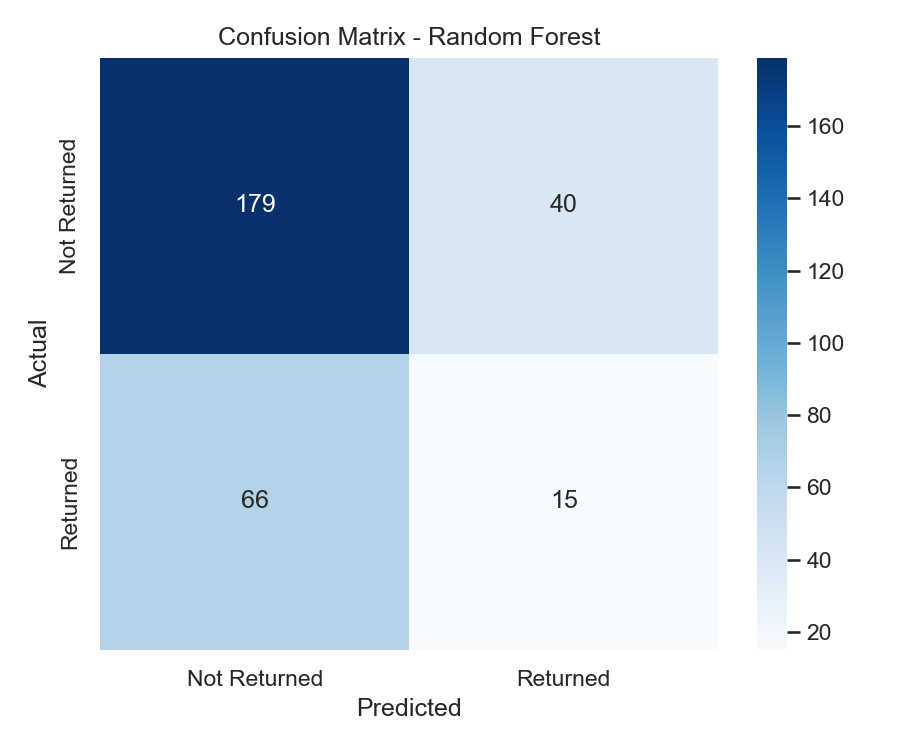
\includegraphics[width=0.55\textwidth]{08_confusion_matrix_best_model.png}
    \end{center}
    \small Model çoğunluk sınıfını yakalar; iade recall düşük (FN=66).
\end{frame}

\begin{frame}{ROC Eğrisi ve Özellik Önemi}
    \begin{columns}
        \column{0.5\textwidth}
        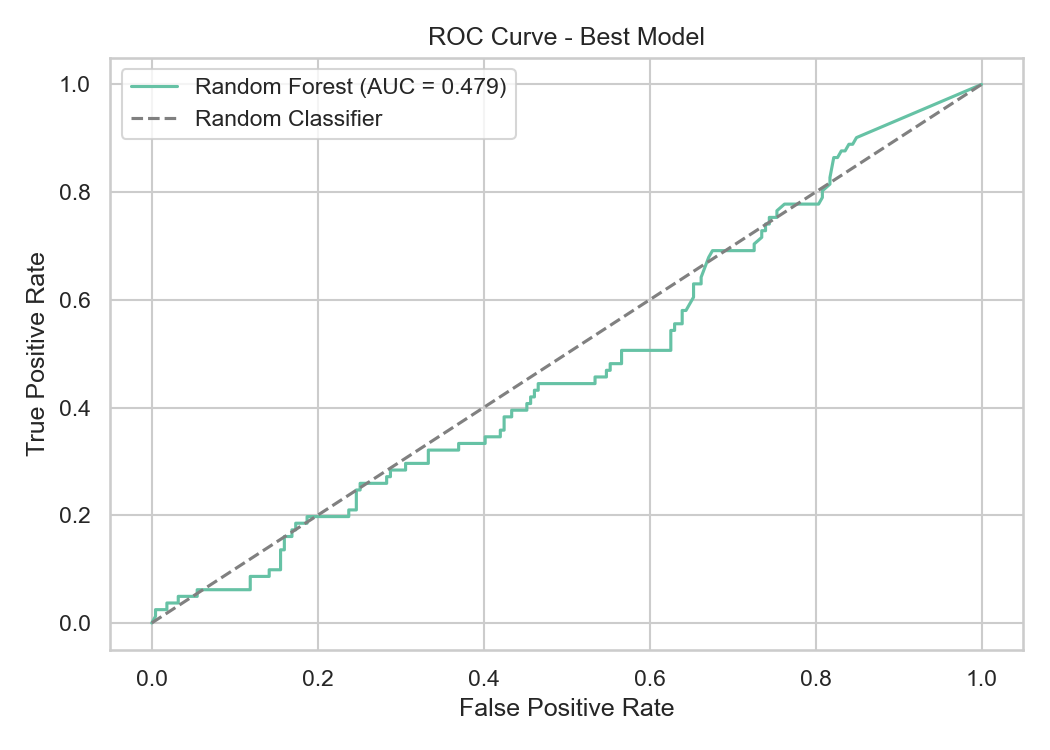
\includegraphics[width=\textwidth]{09_roc_curve_best_model.png}
        \column{0.5\textwidth}
        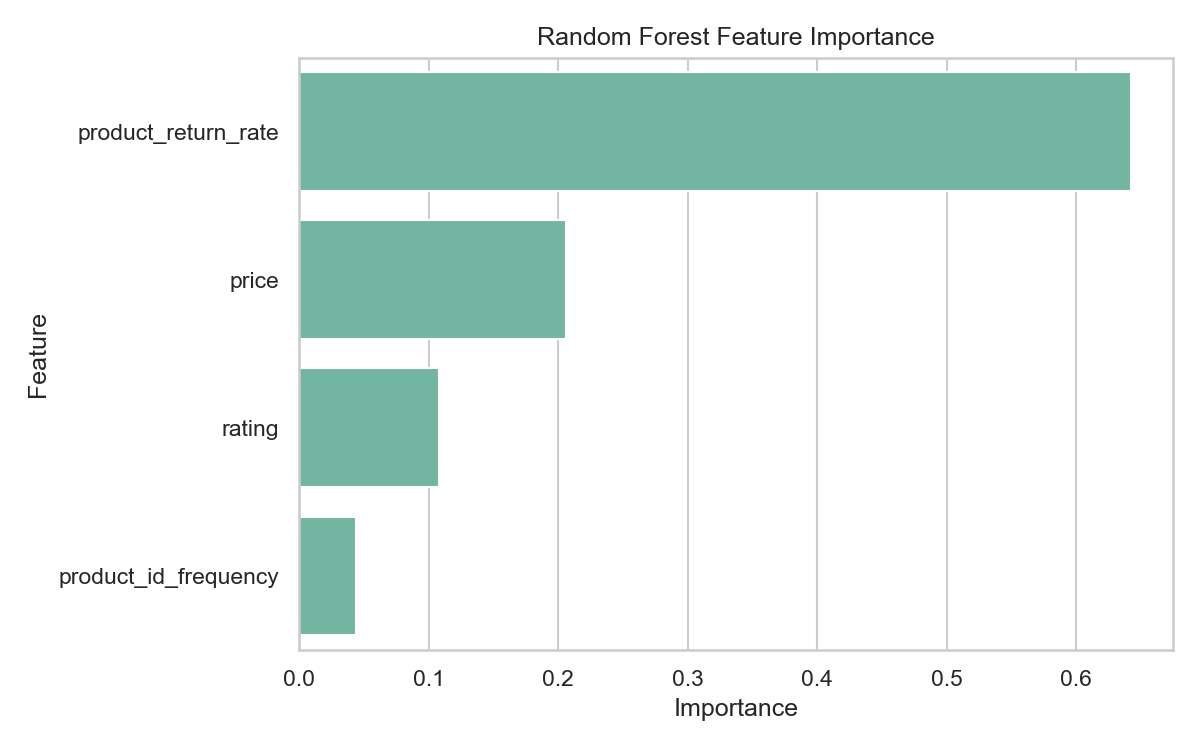
\includegraphics[width=\textwidth]{10_feature_importance_random_forest.png}
    \end{columns}
\end{frame}

% 12. Business
\begin{frame}{İş Yorumu}
    \begin{itemize}
        \item Ürün frekansı ve geçmiş iade oranı güçlü sinyaller
        \item Düşük puanlı siparişler proaktif destek için işaretlenebilir
        \item Yüksek riskli ürünler kalite incelemesine alınabilir
    \end{itemize}
\end{frame}

% 13. Limitations
\begin{frame}{Kısıtlamalar}
    \begin{itemize}
        \item Kategori, indirim, teslimat özellikleri yok
        \item Sınıf dengesizliği recall'u düşürüyor
        \item 78 test ürünü eğitimde görülmedi
        \item Test ROC-AUC sınırlı (0,48)
    \end{itemize}
\end{frame}

% 14. Future work
\begin{frame}{Gelecek Çalışmalar}
    \begin{itemize}
        \item Ek özellikler (yorum, teslimat, promosyon)
        \item SMOTE / maliyet-duyarlı öğrenme
        \item Hiperparametre optimizasyonu
        \item Gerçek zamanlı skorlama
    \end{itemize}
\end{frame}

% 15. Conclusion
\begin{frame}{Sonuç}
    \begin{itemize}
        \item CRISP-DM ile tam veri madenciliği projesi tamamlandı
        \item Random Forest en yüksek CV F1 ile seçildi
        \item Metodoloji: eğitim-only CV, fold-içi encoding, tek seferlik test
        \item E-ticaret iade yönetimi için uygulanabilir içgörüler üretildi
    \end{itemize}
    \vspace{0.5cm}
    \centering
    \textbf{Teşekkürler}
\end{frame}

\end{document}
